\documentclass[spanish, c, dvipsnames]{beamer}

\usepackage[utf8]{inputenc}
%\usepackage[spanish, mexico]{babel}
\usepackage{amsmath}
\usepackage{mathtools}
\usepackage{hyperref}
\usepackage{color}
\usepackage{xcolor}
\usepackage{ragged2e}
\usepackage{mathrsfs}
\usepackage{csquotes}
\usepackage{listings}
\usepackage[scaled]{beramono}
\usepackage[T1]{fontenc}
\usepackage{matlab-prettifier}
\usepackage{graphicx}
\usepackage{booktabs}
\usepackage{gensymb}

\renewcommand{\indent}{\hspace*{2em}}

% \usepackage{tikz}

% \usetikzlibrary{fit, shapes, arrows}

% \usepackage{courier}
% \usepackage{subfigure}
% \usepackage{enumerate}
% \usepackage{algorithmic}
% \usepackage{algorithm}

% \usepackage{listings}
% \usepackage{lstlinebgrd}

\usetheme{Boadilla}
\usefonttheme[onlymath]{serif}

\newcommand{\matlab}[1]{\lstinline[style=Matlab-editor]!#1!}
\newcommand\blfootnote[1]{%
\begingroup
\renewcommand\thefootnote{}\footnote{#1}%
\addtocounter{footnote}{-1}%
\endgroup
}

\lstset
{
    language = Matlab,
    style = Matlab-editor,
    basicstyle = \mlttfamily\scriptsize,
    escapechar = `,
    numbers = left,
    frame = tb,
}

\lstdefinestyle{output}
{
    language = {},
    basicstyle = \mlttfamily\scriptsize,
    escapechar = `,
    numbers = none,
    showtabs = false,
   	showstringspaces = false,
}

\makeatletter
\renewcommand*\env@matrix[1][*\c@MaxMatrixCols c]{%
  \hskip -\arraycolsep
  \let\@ifnextchar\new@ifnextchar
  \array{#1}}
\makeatother

% Sets the templates
\definecolor{navyblue}{RGB}{0, 0, 128}
\definecolor{crimson}{RGB}{128, 16, 0}

\setbeamertemplate{navigation symbols}{}
\setbeamertemplate{headline}{}
\setbeamertemplate{title page}[default][colsep=-4bp,rounded=true]
\setbeamertemplate{footline}[frame number]
\setbeamertemplate{bibliography item}[text]
\setbeamertemplate{theorems}[numbered]

\setbeamercolor{title}{fg=navyblue, bg=white}
\setbeamercolor{frametitle}{fg=navyblue, bg=white}
\setbeamercolor{structure}{fg=navyblue}
\setbeamercolor{button}{fg=white,bg=navyblue}

\setbeamercovered{transparent}

\title{Ajuste de Curvas e Interpolación}
\subtitle{Aplicación de Métodos Numéricos al Ambiente Construido \\ (CV1012)}
\author{
    \texorpdfstring{
        \begin{center}
            Xavier Sánchez Díaz
        \end{center}
    }
    {Xavier Sánchez Díaz}
}

\institute[Tecnológico de Monterrey]{
\includegraphics[scale=0.5]{../img/logo}}
\date{}

\begin{document}

\setlength{\rightskip}{0pt}

\begin{frame}[plain]
    \titlepage        
\end{frame}

\begin{frame}{Outline}
    \tableofcontents
\end{frame}

\section{Continuo y diferenciable}

\begin{frame}{Recuento}{Continuo y diferenciable}

    Hasta el momento hemos revisado los siguientes temas:

    \begin{itemize}
        \itemsep2.5ex
        \item Métodos numéricos para encontrar raíces de ecuaciones no lineales: \pause
        \begin{itemize}
            \item Métodos de intervalos: \textit{bisección}, \textit{falsa posición} \pause
            \item Métodos abiertos: \textit{punto fijo}, \textit{Newton-Raphson}, \textit{secante} \pause
        \end{itemize}
        \item Matrices: \pause
        \begin{itemize}
            \item Operaciones algebraicas con matrices y vectores \pause
            \item Solución de sistemas de ecuaciones lineales usando eliminación
        \end{itemize}
    \end{itemize}

\end{frame}

\begin{frame}{¿Cómo ha sido el proceso?}{Continuo y diferenciable}
    Hasta ahora, nos dan una ecuación \textit{bonita} y nos dicen qué hacer o qué debemos encontrar en ella. \blfootnote{\url{https://falseknees.com/249.html}}
    Sin embargo, la vida no es así de fácil\dots
    \begin{center}
        
\includegraphics[width=0.48\textwidth]{beautifulbutfragile.png}
    \end{center}

\end{frame}

\section{Discreto y aproximable}

\begin{frame}{La realidad es distinta}{Discreto y aproximable}
    En ingeniería usualmente tomamos mediciones, y a partir de ello tratamos de hacer generalizaciones. \pause

    \bigskip

    Para ello, tenemos herramientas como el \alert{ajuste de curvas}, en donde tratamos de encontrar una \textbf{función} que \textit{describa} el comportamiento de nuestras \textbf{observaciones}.
\end{frame}

\begin{frame}{Generalizando}{Discreto y aproximable}
    A partir de datos\dots

    \begin{center}
        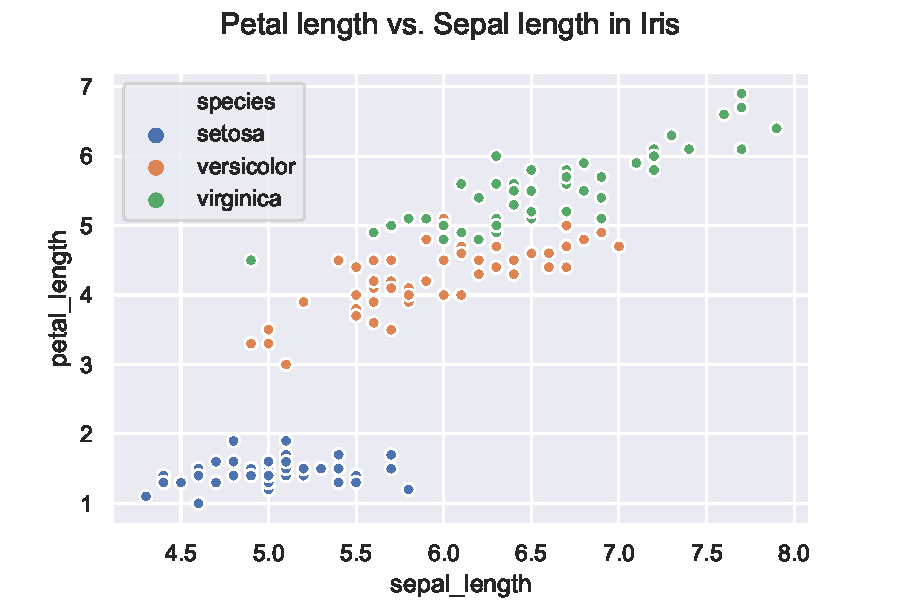
\includegraphics[width=0.7\textwidth]{scatter.pdf}
    \end{center}
    

\end{frame}

\begin{frame}{Generalizando}{Discreto y aproximable}

    \dots generalizamos.

    \begin{center}
        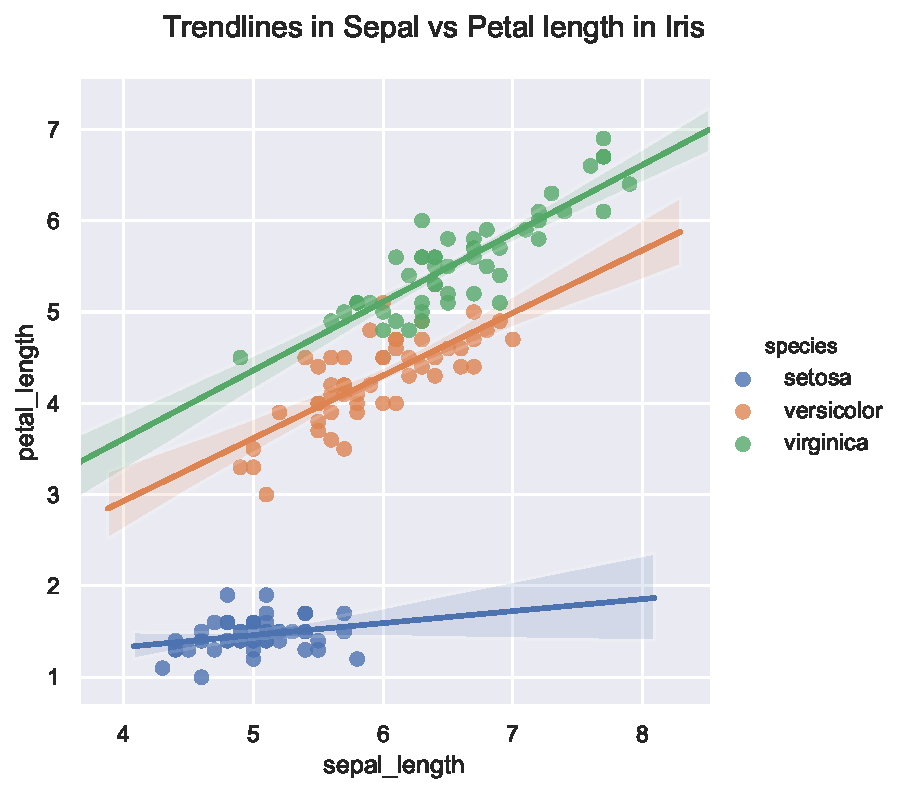
\includegraphics[width=0.62\textwidth]{regplot.pdf}
    \end{center}
    
\end{frame}

\section{Estadística descriptiva básica}

\begin{frame}{Nuestras herramientas}{Estadística descriptiva básica}

Para poder generalizar a partir de una \alert{muestra} de datos, necesitamos saber \textit{más o menos} cómo se comportan. \pause

\bigskip

En este caso, podemos calcular a partir de nuestra \textbf{muestra} algunas \alert{estadísticas} que nos ayuden a comprender este comportamiento. \pause

\begin{itemize}[<+->]
    \item ¿Cuántos datos tenemos?
    \item ¿Cuál es el máximo valor? ¿Cuál es el mínimo?
    \item ¿Qué tan separados están los datos?
    \item ¿Alrededor de qué valor se concentra la mayoría de los datos?
    \item ¿Cuál es el dato más común?
\end{itemize}
\end{frame}

\begin{frame}{Media aritmética}{Estadística descriptiva básica}
    La \alert{media aritmética} (mejor conocida como \textbf{promedio}) es una excelente manera de obtener información inmediata sobre el comportamiento \textit{promedio} (duh) de nuestra muestra:

    \bigskip

    \begin{block}{Media}
        $$\bar{y} = \frac{\sum y_i}{n}$$
    \end{block}

    \bigskip

    donde $n$ es el \alert{tamaño de la muestra} (o sea, cuántos datos tenemos), y $y_i$ es el $i$-ésimo elemento en nuestra muestra.
\end{frame}

\begin{frame}{Mediana}{Estadística descriptiva básica}
    Otra medida de centralidad importante es la \alert{mediana}, que es el valor de \textbf{en medio} de los datos \textbf{cuando están ordenados}. \pause

    \bigskip

    Es importante recalcar que \textbf{la media} y \textbf{la mediana} \alert{no son lo mismo}, aunque \textbf{a veces pueden ser idénticas}. \pause

    \bigskip

    \begin{itemize}[<+->]
        \itemsep2ex
        \item \textit{El sueldo promedio del mexicano} hace referencia a la \alert{media} de los sueldos: sumas todos los sueldos y los divides entre los entrevistados para saber \textit{lo que esperas que gane un mexicano comúnmente}.
        \item \textit{El sueldo del mexicano promedio} hace referencia a la \alert{mediana} de los sueldos: ordenas todos los sueldos, y tomas el de en medio para saber \textit{lo que esperas que gane un mexicano de clase media}.
    \end{itemize}
\end{frame}

\begin{frame}{Moda}{Estadística descriptiva básica}
    Otra medida comúnmente empleada es la \alert{moda}, que viene a ser el dato que \textbf{más se repite} en la \textbf{muestra}. \pause

    \bigskip

    Siguiendo con nuestro ejemplo anterior, la \textbf{moda} vendría a representar \textit{lo que gana la mayoría de los mexicanos}.
\end{frame}

\begin{frame}{Midiendo la dispersión}{Estadística descriptiva básica}
    La \alert{desviación estándar} es la medida de \textit{dispersión} más común:

    \begin{block}{Desviación estándar}
        $$S_y = \sqrt{\frac{S_t}{n-1}}$$
    \end{block}

    donde $S_t$ es la \alert{suma total de los cuadrados de los residuales} entre cada dato y la media:

    $$S_t = \sum (y_i - \bar{y})^2$$

    Otra medida de dispersión muy utilizada es la \alert{varianza}, que es igual \textbf{al cuadrado de la desviación estándar}.
\end{frame}

\section{Ajuste de curvas}

\begin{frame}{Regresión lineal}{Ajuste de Curvas}
    Como vimos anteriormente, queremos obtener información a partir de nuestras mediciones, para poder \textbf{generar} un \alert{modelo matemático} (o sea una función).

    \bigskip

    ¿Cuál es la manera más sencilla de unir dos puntos?

    \begin{center}
        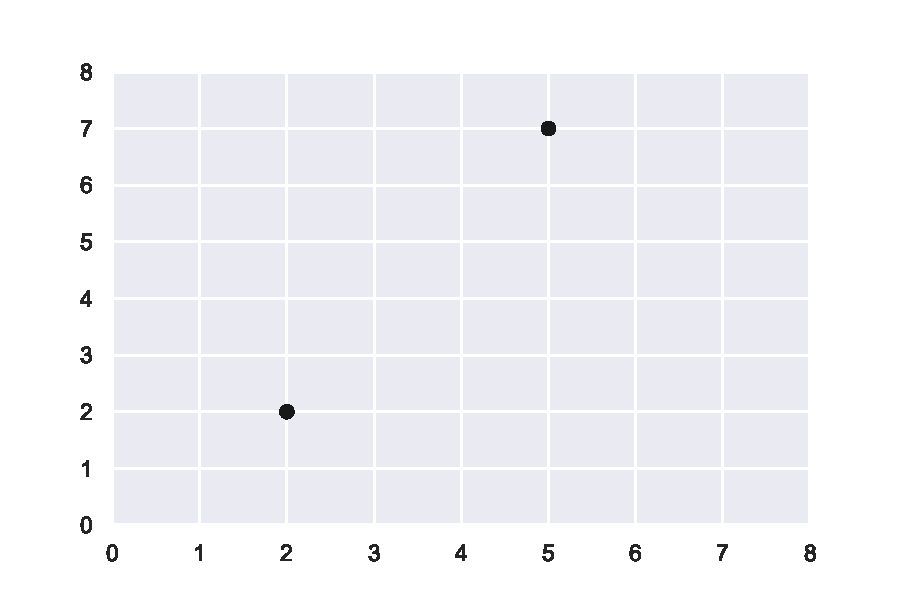
\includegraphics[width=0.6\textwidth]{dots.pdf}
    \end{center}
\end{frame}

\begin{frame}{Regresión lineal}{Ajuste de Curvas}
    
    ¿Cómo se ve una línea recta si usamos dos puntos? \bigskip

    \begin{center}
        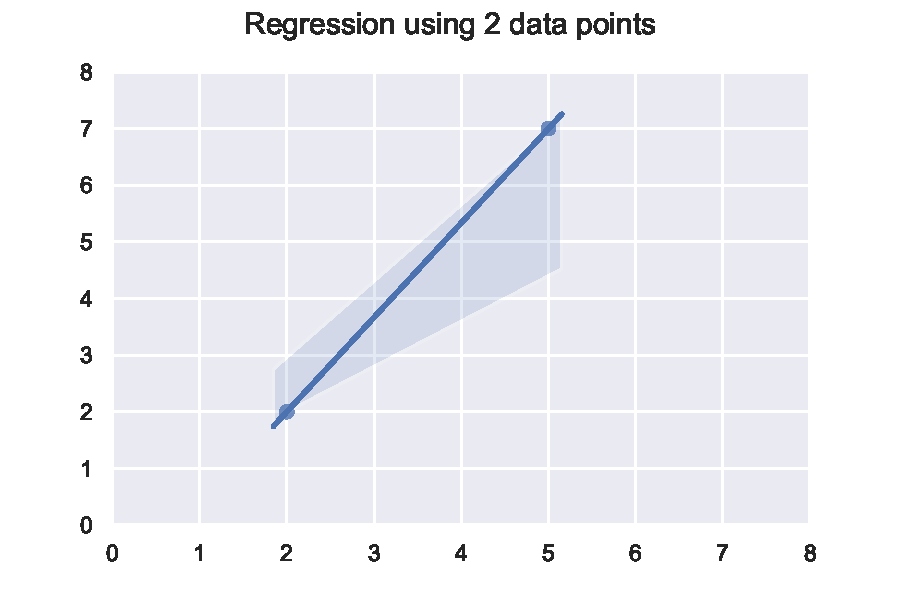
\includegraphics[width=0.7\textwidth]{reg01.pdf}
    \end{center}    

\end{frame}

\begin{frame}{Regresión lineal}{Ajuste de Curvas}
    
    ¿Y si agregamos otra medición? \bigskip

    \begin{center}
        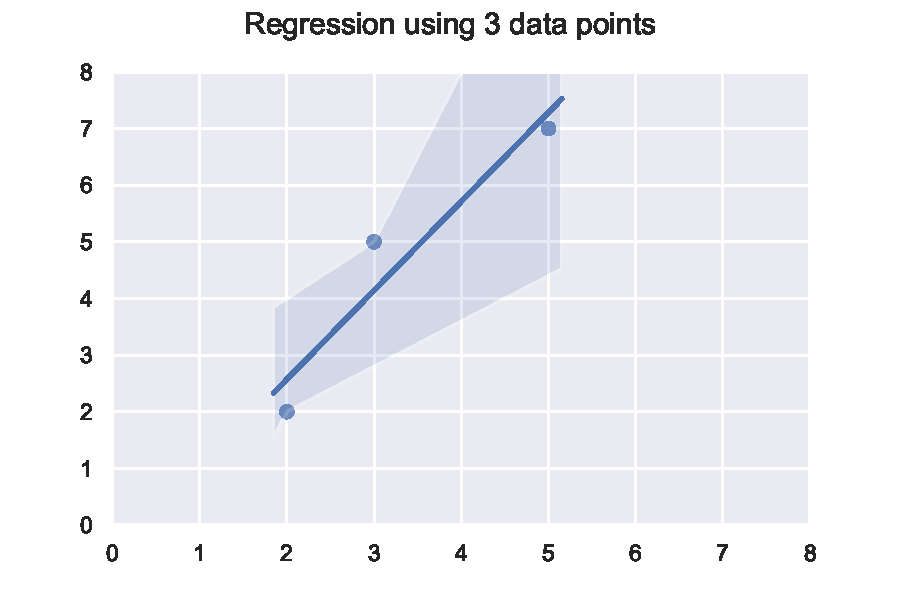
\includegraphics[width=0.7\textwidth]{reg02.pdf}
    \end{center}
\end{frame}

\begin{frame}{Regresión lineal}{Ajuste de Curvas}
    
    ¿Y si agregamos otra más? \bigskip

    \begin{center}
        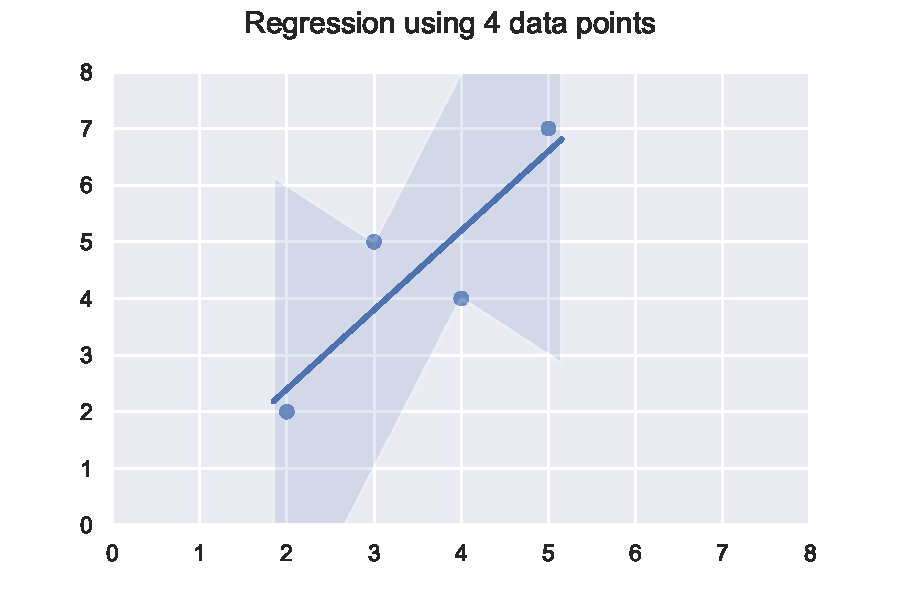
\includegraphics[width=0.7\textwidth]{reg03.pdf}
    \end{center}
\end{frame}

\begin{frame}{Mínimos cuadrados}{Ajuste de curvas}
    ¿Cómo sabemos si la línea que hicimos es la \textit{mejor} aproximación que tenemos para la tendencia? \pause

    \bigskip

    \begin{itemize}[<+->]
        \itemsep2.5ex
        \item Podemos contar a cuántos puntos le atinamos y cuántos no
        \item Podemos revisar por cuánto fallamos en cada punto y sumarlo
        \item Podemos revisar por cuánto fallamos en cada punto y sacarle valor absoluto
        \item \alert<6>{Podemos revisar por cuánto fallamos en cada punto, elevarlo al cuadrado, y sacar un promedio}
    \end{itemize}
\end{frame}

\begin{frame}{Mínimos cuadrados}{Ajuste de curvas}
    Para obtener la ecuación de una recta necesitamos dos elementos:

    $$y = {\color{blue} a_1} x + {\color{ForestGreen} a_0}$$

    \begin{block}{Pendiente}
        $$a_1 =  \frac{n \sum x_i y_i - \sum x_i \sum y_i}{n \sum x_i^2 - (\sum x_i)^2}$$
    \end{block}

    \begin{exampleblock}{Ordenada al origen}
        $$a_0 = \bar{y} - a_1 \bar{x}$$
    \end{exampleblock}

\end{frame}

\begin{frame}{Calidad de la regresión}{Ajuste de Curvas}
    
    Para revisar la \textbf{calidad} de nuestra regresión, podemos usar una estadística llamada $r^2$.

    \begin{block}{Calculando $r^2$}
        $$r^2 = \frac{S_t - S_r}{S_t}$$
    \end{block}

    Donde $S_t$ es la suma de todos los cuadrados de los residuales con la media:
    
    $$S_t = \sum\limits_{i=1}^n (y_i - \bar{y})^2$$

    y $S_r$ es la suma de todos los cuadrados de los residuales con nuestra regresión:

    $$S_r = \sum\limits_{i=1}^n (y_i - a_0 - a_1 x_i)^2$$
    
\end{frame}

\begin{frame}{Pendientes}{Interpolación}
    ¿Cuántas pendientes tiene la siguiente \textsl{función}?

    \bigskip

    \begin{center}
        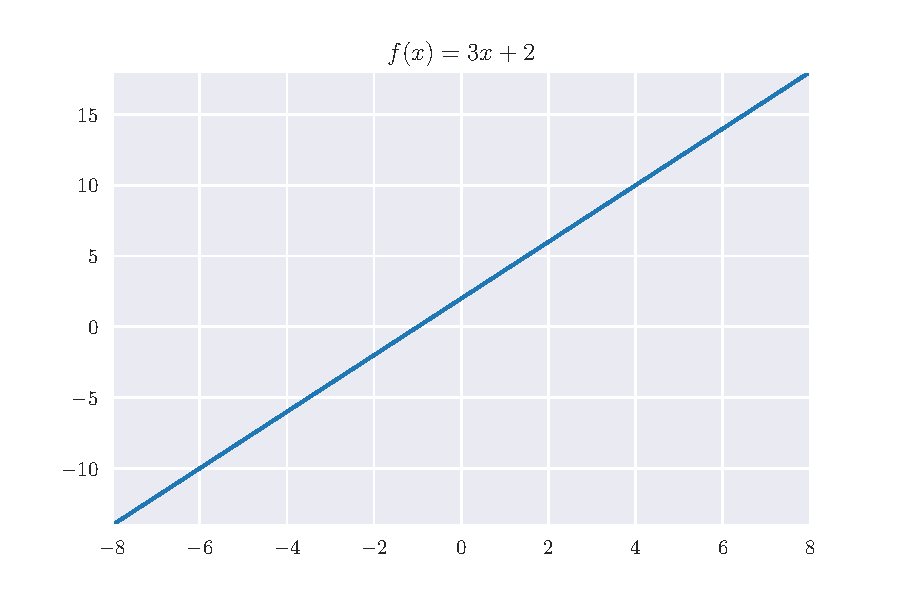
\includegraphics[width=0.75\textwidth]{linear.pdf}
    \end{center}

\end{frame}

\begin{frame}{Pendientes}{Interpolación}
    ¿Cuántas pendientes tiene la siguiente \textsl{función}?

    \bigskip

    \begin{center}
        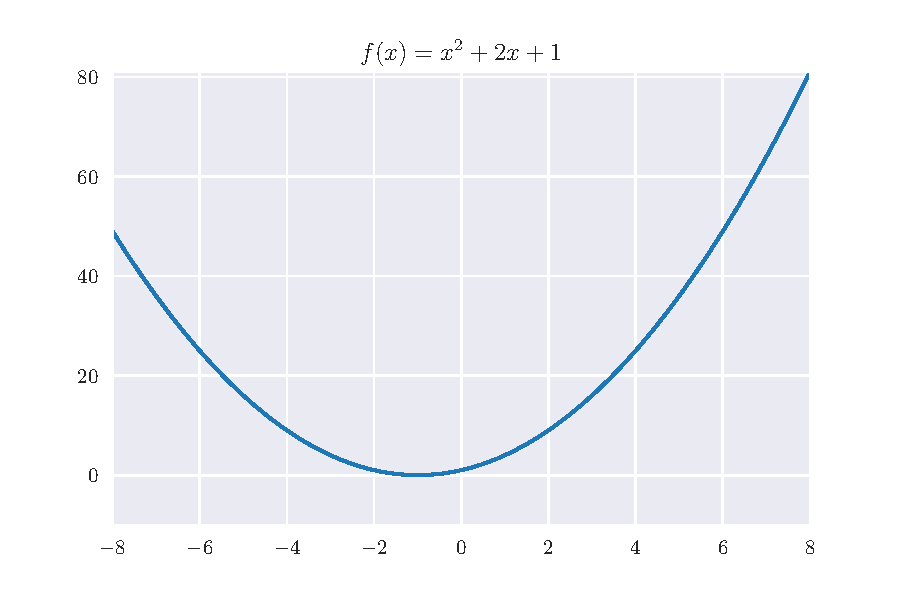
\includegraphics[width=0.75\textwidth]{quad.pdf}
    \end{center}

\end{frame}

\begin{frame}{Pendientes}{Interpolación}
    ¿Cuántas pendientes tiene la siguiente \textsl{función}?

    \bigskip

    \begin{center}
        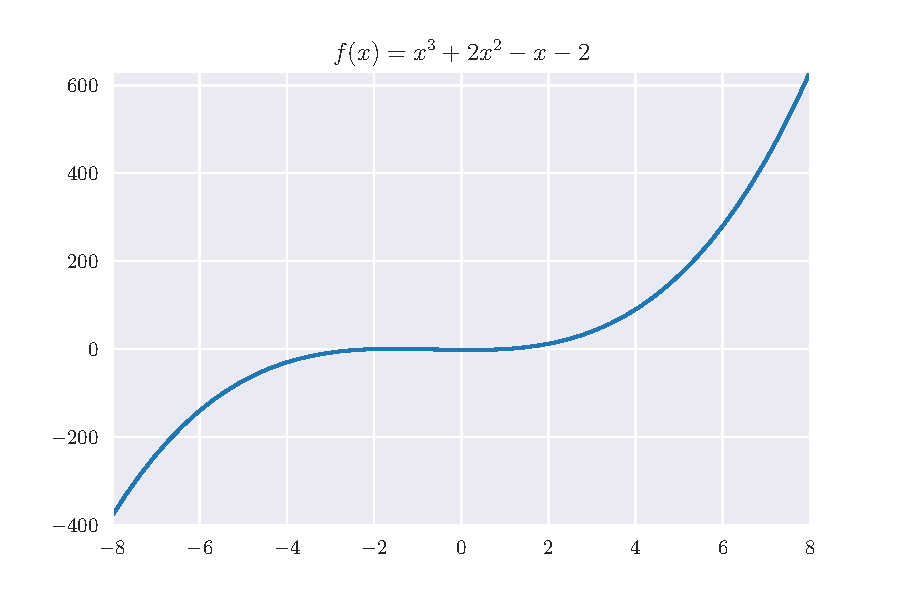
\includegraphics[width=0.75\textwidth]{cubic.pdf}
    \end{center}

\end{frame}

\begin{frame}{Ajuste polinomial}{Interpolación}
    
    Como ya vimos, se puede ajustar una función que \textsl{aproxime} los puntos.
    Sin embargo, también se pueden usar métodos para encontrar una función que pase \textbf{exactamente} por cada uno de ellos. \pause

    \bigskip

    \begin{itemize}[<+->]
        \item Para unir $n$ puntos, siempre se existirá un \alert{polinomio} de \textbf{grado} $n-1$ que describa su comportamiento exacto
        \item Calcular este polinomio para grados muy altos es computacionalmente \textbf{costoso}
        \item Para grados muy altos, el \textbf{error} en los extremos tiende a ser mucho más grande
    \end{itemize} \pause
    
    \begin{center}
        \itshape
        Story time:\\
        Overfitting
    \end{center}

\end{frame}

\begin{frame}{El concepto de interpolación}{Interpolación}
    
    \alert{Interpolar} hace referencia a obtener puntos \textbf{intermedios} a partir de mediciones dadas:

    \bigskip
    \begin{columns}
        \begin{column}{0.5\textwidth}
            \begin{center}
                \begin{table}[H]
                    \begin{tabular}{lr}
                    \hline
                    \textbf{t (s)} & \textbf{v (m/s)} \\ \hline
                    0              & 0.00             \\
                    2              & 16.42            \\
                    4              & 27.8             \\
                    6              & 35.68            \\
                    8              & 41.14            \\
                    10             & 44.92            \\
                    12             & 47.54            \\
                    $\infty$       & 53.44            \\ \hline
                    \end{tabular}
                \end{table}
            \end{center}
        \end{column}
        \begin{column}{0.5\textwidth}
            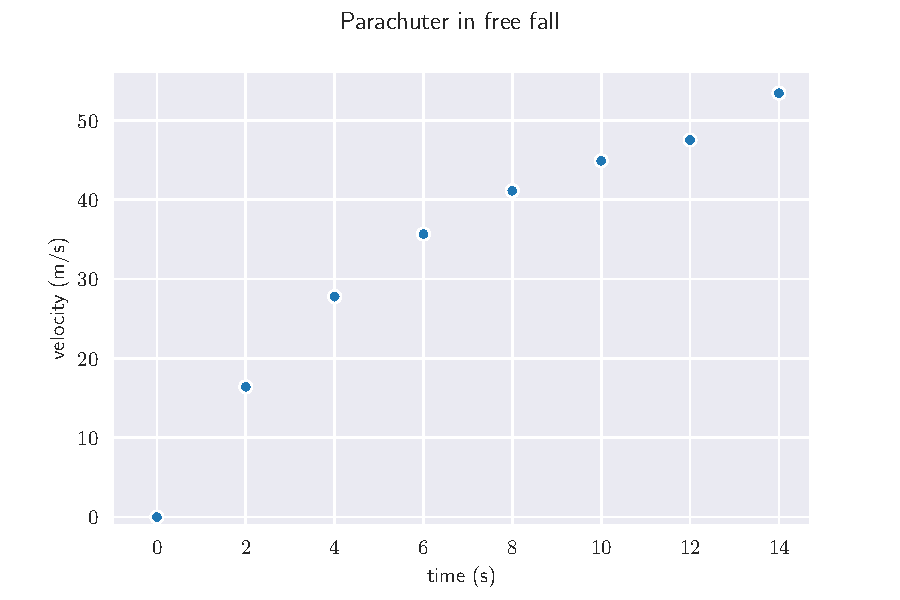
\includegraphics[width=\columnwidth]{parachuter.pdf}
        \end{column}
    \end{columns}

    \bigskip
    ¿Cuál será la velocidad a los 5 segundos?
\end{frame}

\begin{frame}{Interpolación lineal}{Interpolación}

    La \alert{interpolación lineal} (o clásica) consiste en unir entre puntos con líneas rectas.

    \bigskip

    \begin{center}
        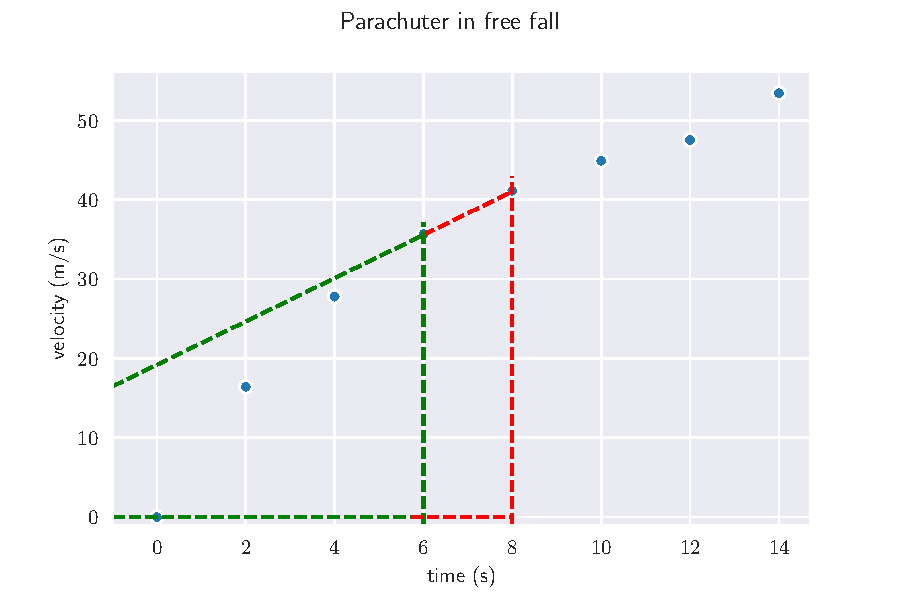
\includegraphics[width=0.65\textwidth]{inter01.pdf}
    \end{center}

\end{frame}

\begin{frame}{Interpolación con mínimos cuadrados}{Interpolación}

    También podemos \alert{interpolar por mínimos cuadrados} linealmente, evaluando $f(5)$:

    $$f(x) = 3.49107143 x + 8.93$$

    \begin{center}
        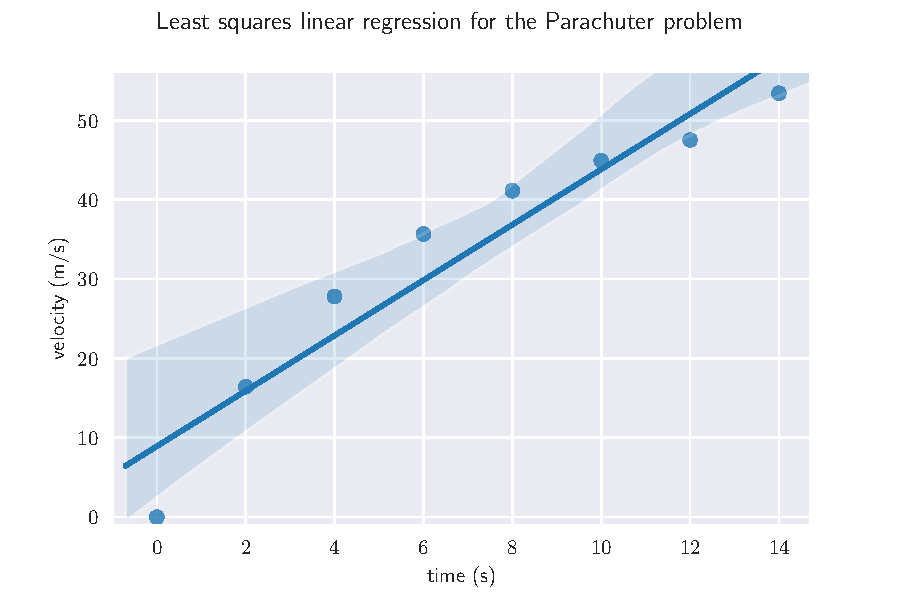
\includegraphics[width=0.65\textwidth]{inter02.pdf}
    \end{center}

\end{frame}

\begin{frame}{Interpolación con mínimos cuadrados}{Interpolación}

    O con un polinomio de segundo grado:

    $$f(x) = -0.244375 x^2 + 6.91232143 x + 2.0875$$

    \begin{center}
        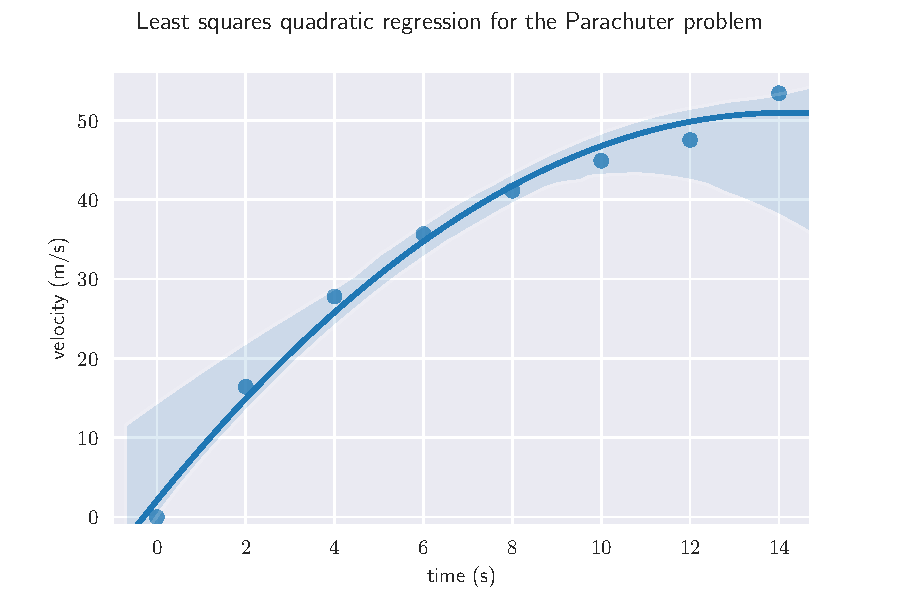
\includegraphics[width=0.65\textwidth]{inter03.pdf}
    \end{center}

\end{frame}

\begin{frame}{Interpolación con mínimos cuadrados}{Interpolación}

    O con un polinomio de grado 7 (que es terrible):
    \begin{equation*}
        \begin{split}
            f(x) = 0.000006.23139881 x^7 -0.000261718750 x^6 + 0.00439322917 x^5 \\
            -0.00384635417 x^4 + 0.0212750000 x^3 -1.23945833 x^2 \\
            + 10.0833095 x -0.0000000000003.01457752
        \end{split}
    \end{equation*}

    \begin{center}
        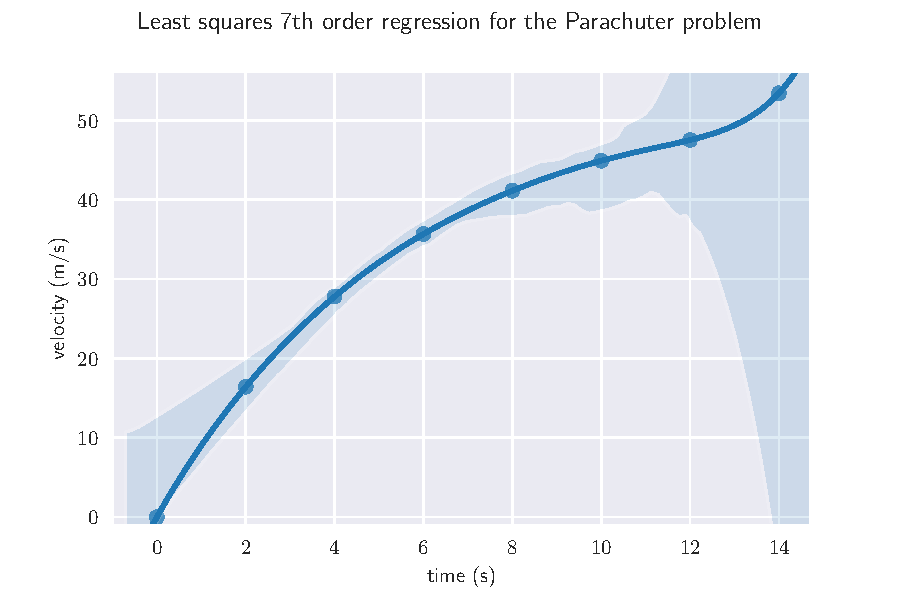
\includegraphics[width=0.59\textwidth]{inter04.pdf}
    \end{center}

\end{frame}


%deg 1
% 
% 
% 0.000006.23139881 x^7 -0.000261718750 x^6 + 0.00439322917 x^5 -0.00384635417 x^4 + 0.0212750000 x^3 -1.23945833 x^2 + 10.0833095 x -0.0000000000003.01457752
% Específicamente, la regla 3 puede verse como $R_i = R_i - \frac{a_{ik}}{a_{jk}}R_j$.

% Los robots
% why is it important
% does it exist in math?
% how to represent it
% how to represent it in matlab
% practical cases

% \section*{Referencias}

% \begin{frame}[t]{Referencias}
    % \nocite{bibID01}
    % \nocite{bibID02}

    % \bibliographystyle{IEEE}
    % \bibliography{biblio}
% \end{frame}

\end{document}